\documentclass{article}
\usepackage{graphicx} % Required for inserting images
\usepackage{hyperref}
\usepackage{xcolor}




\title{Interfaz web FAB}
\author{Ale Serrano}
\date{May 2025}

\begin{document}

\maketitle

\section{Introduction}

En esta ocasión vamos a crear una interfaz web con nuestro script fab, aunque hemos quitado el hardcodeo del csv y convertido fab en una clase. 

\section{FAB}
En esta tarea había dos requisitos, quitar el hardcodeo y convertir fab en una clase. Para ello he hecho este script: \href{fabweb.py}{\underline{\textcolor{blue}{fabweb.py}}}


\section{Aplicación web}
Con lo visto en clase y lo investigado por nuestra cuenta, la primera parte es crear el entorno virtual y descargar las dependencias necesarias para la tarea que en este caso es "flask". 

\begin{figure}
    \centering
    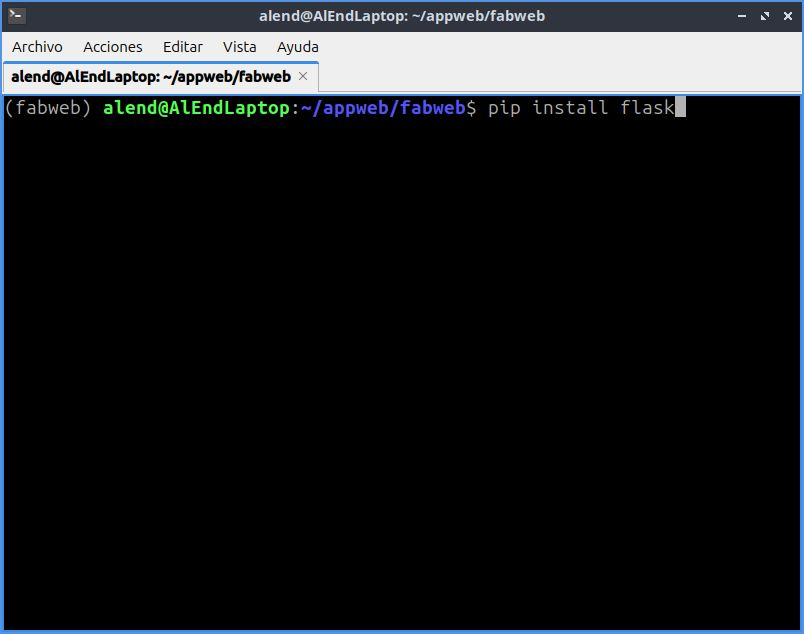
\includegraphics[width=0.5\linewidth]{Images/fabweb1.jpg}
    \caption{pip install flask}
    \label{fig:enter-label}
\end{figure}

Tras esto nos ponemos con el archivo de la app.

\subsection{App.py}
Lo primero serán los "imports", en este caso tendremos que importar el sistema ("os"), de flask importaremos "Flask", "request", "abort" y "render\_template" y por último la clase "fab" del script anterior. Para esta aplicación vamos a crear varias rutas, la página principal se encargará de seleccionar el archivo que queremos ver, que en este caso solo esta el de "envivo.csv". Tras seleccionar el archivo, queremos que se redirija a otra página donde nos muestre la tabla ya procesada por "fab" y todo esto sin olvidar tener en cuenta los errores.\

Tras pedirle a chatgpt un css bonito para las páginas, quedaria algo así.
Mi próxima idea es poder hacer que el usuario suba el archivo .csv y de este formato y que haga lo mismo pero eso será en el próximo capitulo.

\begin{figure}
    \centering
    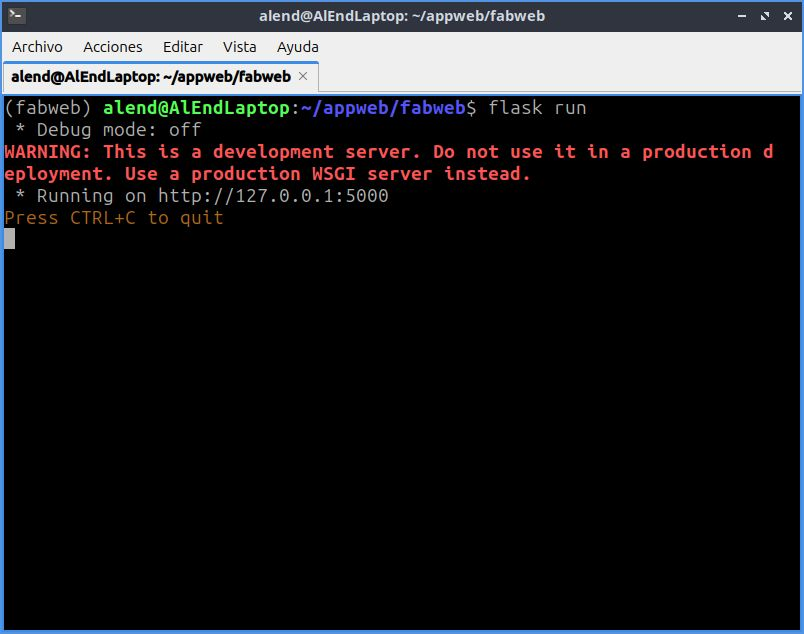
\includegraphics[width=0.5\linewidth]{Images/fabweb2.jpg}
    \caption{Flask run para abrir el localhost}
    \label{fig:enter-label}
\end{figure}

\begin{figure}
    \centering
    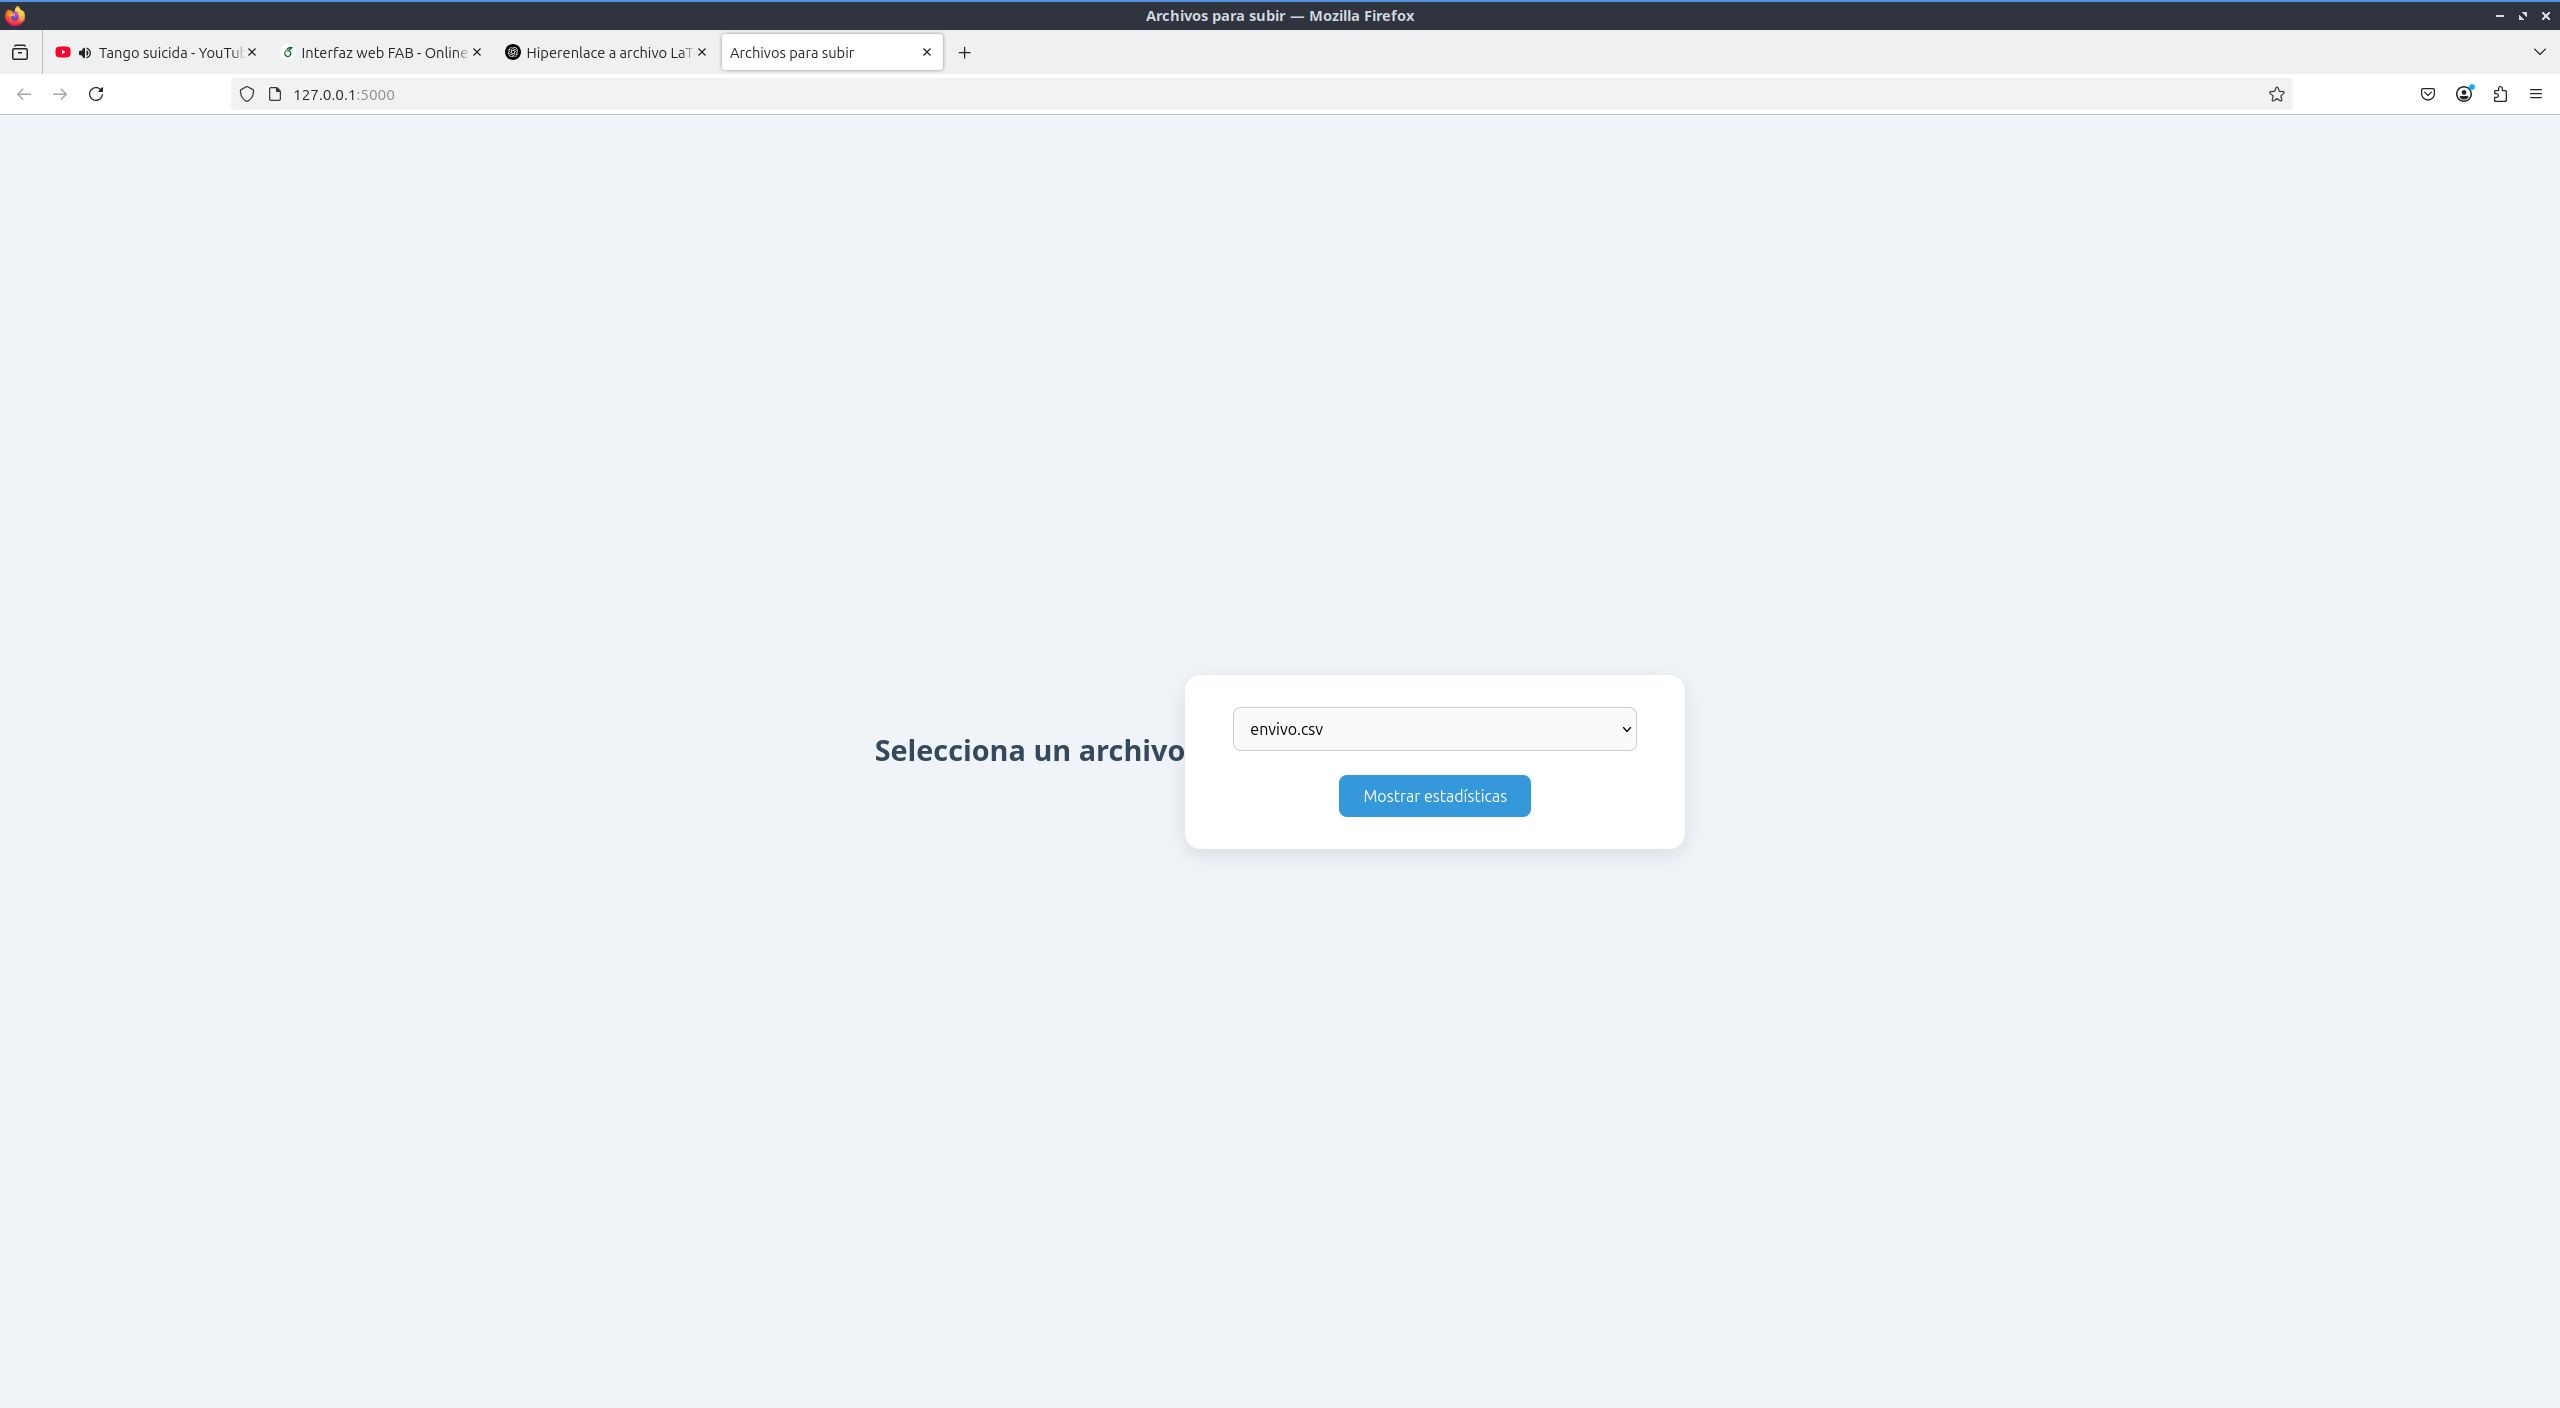
\includegraphics[width=0.5\linewidth]{Images/fabweb3.jpg}
    \caption{página para seleccionar archivo}
    \label{fig:enter-label}
\end{figure}

\begin{figure}
    \centering
    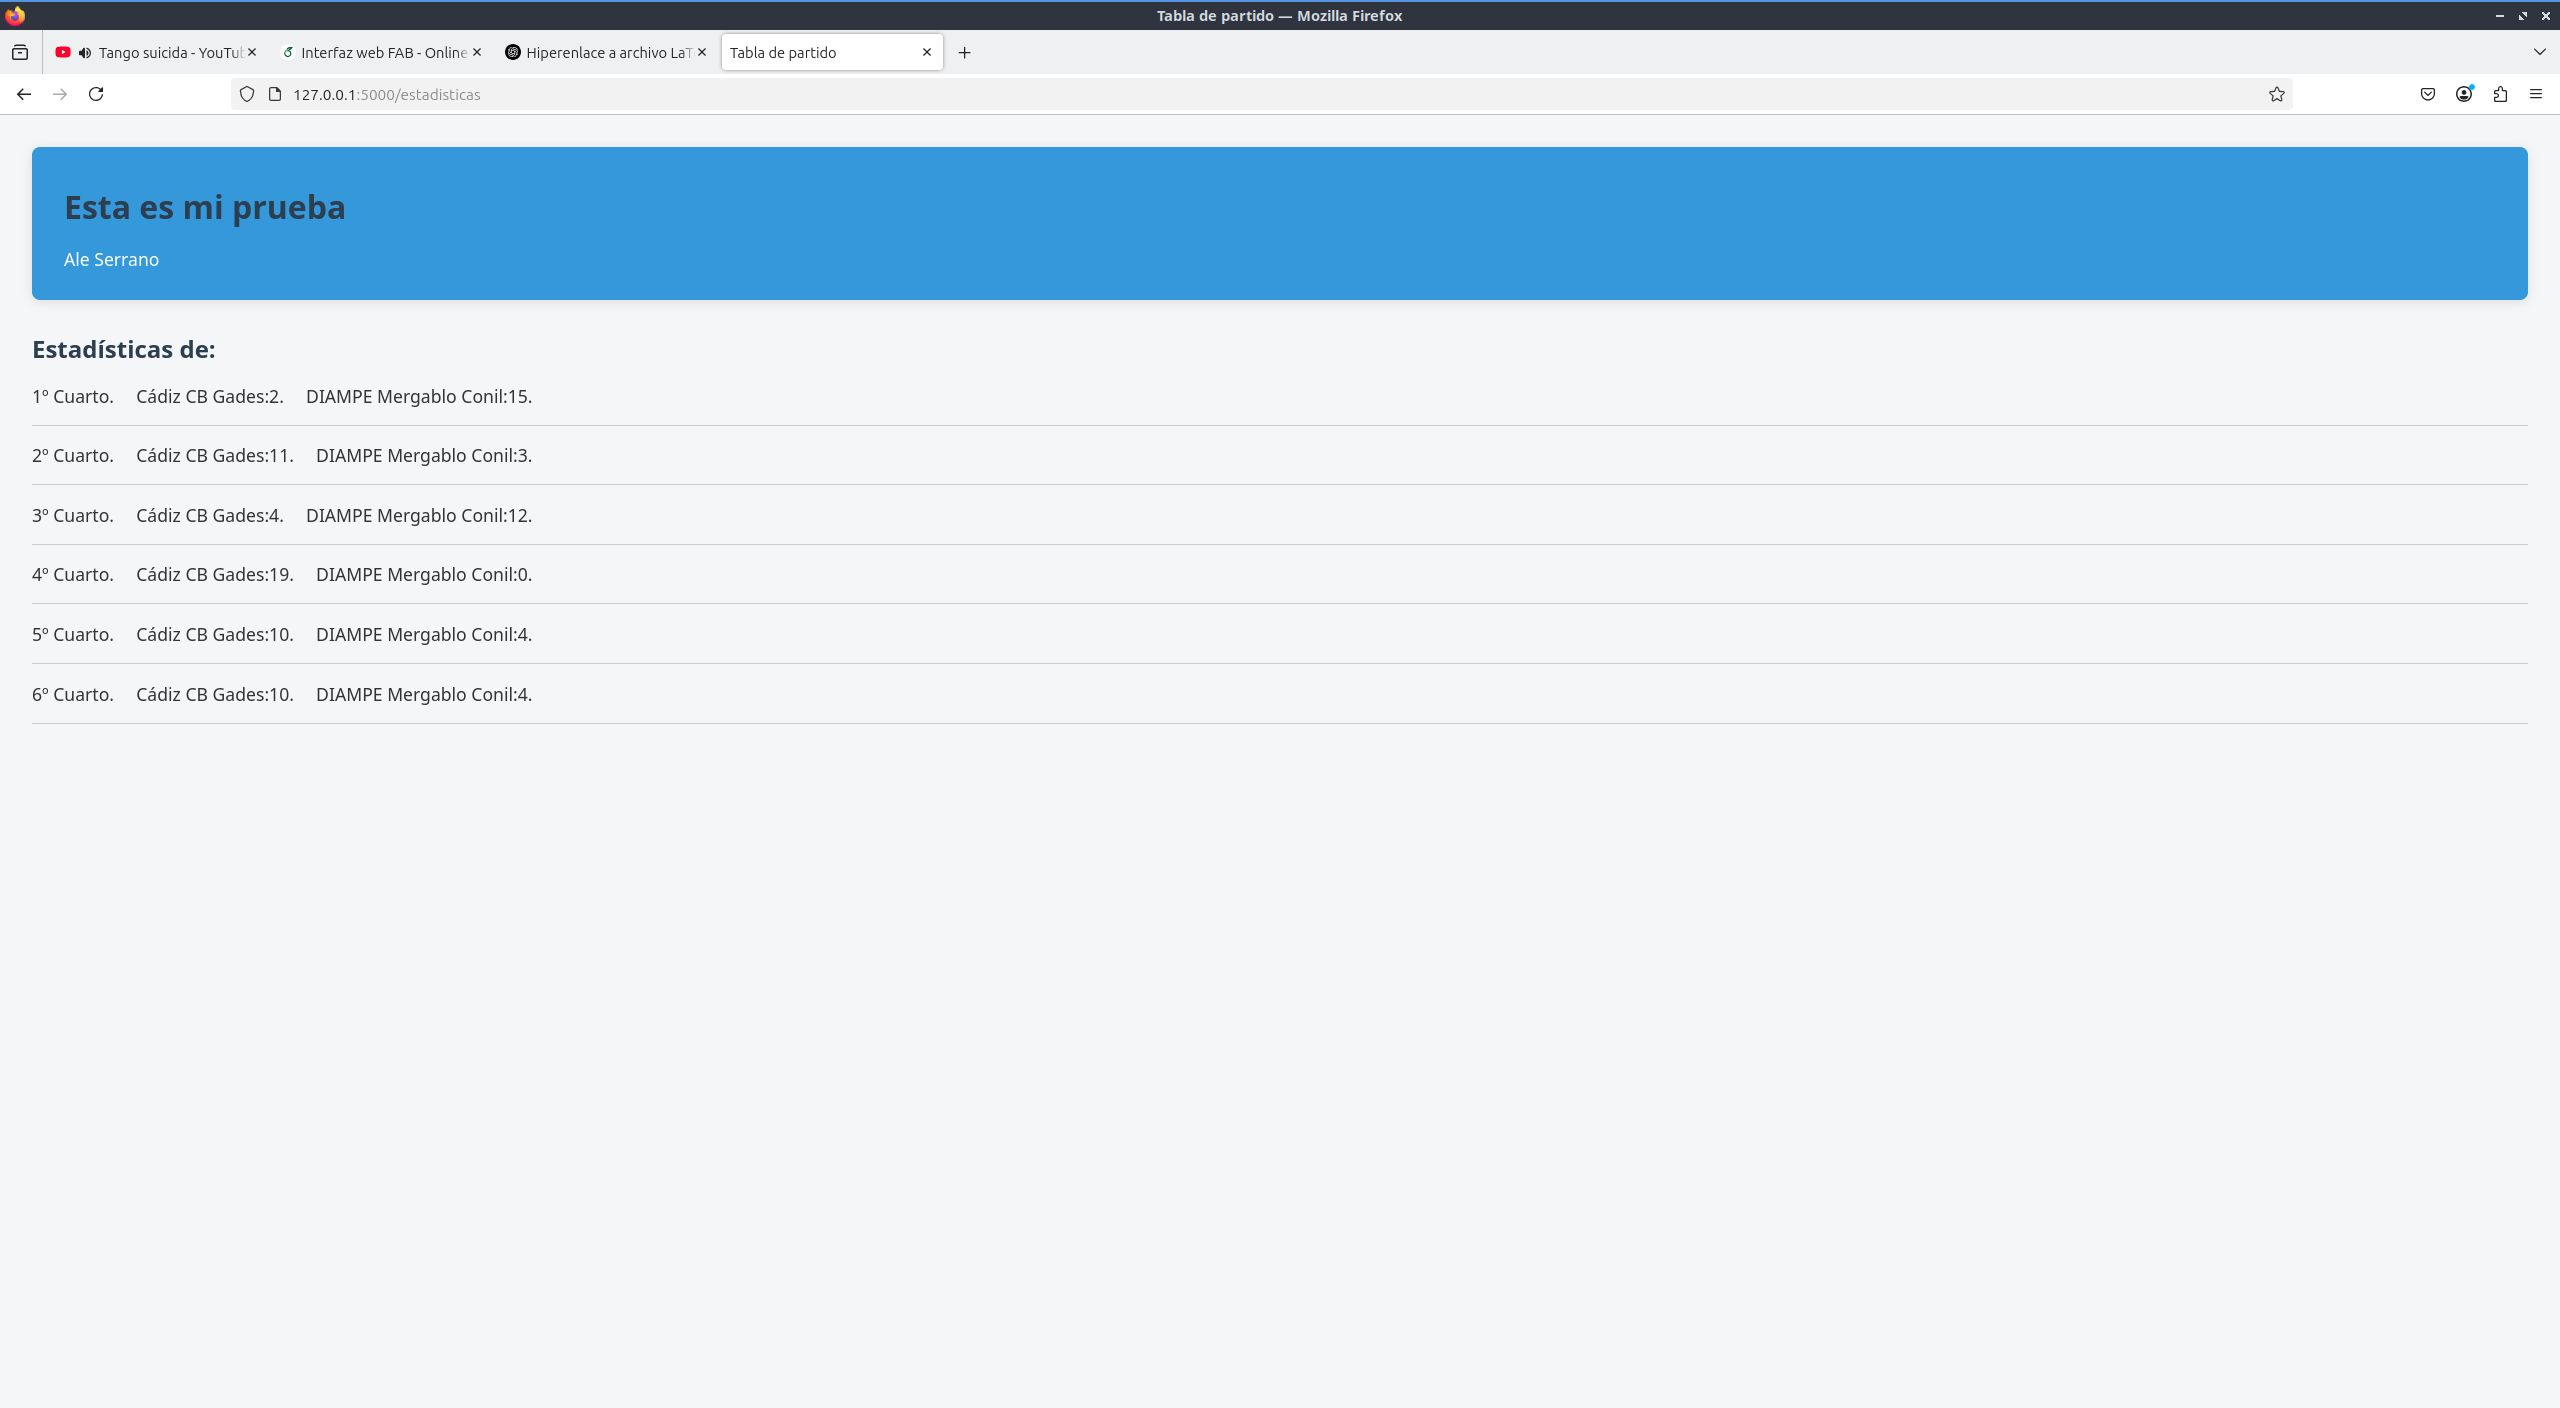
\includegraphics[width=0.5\linewidth]{Images/fabweb4.jpg}
    \caption{resultados de envivo.csv}
    \label{fig:enter-label}
\end{figure}

\end{document}


